\documentclass{article}
\usepackage[T2A]{fontenc}
\usepackage[utf8]{inputenc}
%\usepackage[russian]{babel}
\usepackage{amsmath}
\usepackage{amsthm}
\usepackage{mathtools}
\usepackage{algorithm}
\usepackage{algorithmicx}
\usepackage{algpseudocode}
\usepackage{tikz}

\DeclarePairedDelimiter\abs{\lvert}{\rvert}%
\DeclarePairedDelimiter\norm{\lVert}{\rVert}%

% Swap the definition of \abs* and \norm*, so that \abs
% and \norm resizes the size of the brackets, and the 
% starred version does not.
\makeatletter
\let\oldabs\abs
\def\abs{\@ifstar{\oldabs}{\oldabs*}}
%
\let\oldnorm\norm
\def\norm{\@ifstar{\oldnorm}{\oldnorm*}}
\makeatother
%

\providecommand\given{} % so it exists
\newcommand\SetSymbol[1][]{
	\nonscript\,#1\vert \allowbreak \nonscript\,\mathopen{}}

\DeclarePairedDelimiterX\Set[1]{\lbrace}{\rbrace}%
{ \renewcommand\given{\SetSymbol[\delimsize]} #1 }

\newcommand{\pd}[2]{
	\frac{\partial{#1}}{\partial{#2}}
}

\newcommand{\ppd}[1]{
	\frac{\partial}{\partial{#1}}
}

\newcommand{\mean}[3]{
	\frac{1}{#2} \sum_{#1 = 1}^{#2}{#3}
}

\newcommand{\score}[1]{
	\textrm{score}(#1)
}

\newcommand{\pa}[1]{Pa(#1)}

\newcommand{\affnodes}[1]{
	\textrm{Aff}(#1)	
}

\newcommand{\addedge}[1]{
	\textrm{Add}(#1)	
}

\newcommand{\rmedge}[1]{
	\textrm{Del}(#1)
}

\newcommand{\revedge}[1]{
	\textrm{Rev}(#1)
}

\newcommand{\bigO}[1]{
	\mathcal{O}{(#1)}
}

\newcommand{\graph}[1]{
	\mathcal{#1}
}

\newcommand{\var}[1]{{\ttfamily#1}}% variable

\newcommand{\ops}[1]{
	\textrm{ops}(#1)
}

\newcommand{\argmin}{\operatornamewithlimits{argmin}}
\newcommand{\argmax}{\operatornamewithlimits{argmax}}

\author{Dmitry Lunin}
\title{Bayesian Networks}
\begin{document}
\maketitle

\section{Overview}
\subsection{Definition}

\subsection{Workflow}
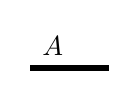
\begin{tikzpicture}[line width=2pt]
\draw (0,0) node [above right]  {$A$} -- (1,0);

\end{tikzpicture}

\section{Structure Learning}
\subsection{Introduction}
\paragraph{The task} The aim of structure learning is to identify the Bayesian network structure (i.e. the graph) using data. 

\paragraph{Applications}

The first application is knowledge discovery. We can use structure learning to find out (in)dependencies between variables in the data, or test our prior assumptions about them, obtaining better understanding of the data and the domain of knowledge. 

The second application is off-the-shelf machine learning. In order to apply Bayesian network methods to a problem, firstly one needs to build a Bayesian network, which may require significant effort and domain expertise. On the other hand, many machine learning methods, for example random forests can be applied immediately, yielding adequate results which can be improved later by fine-tuning parameters. Advanced structure learning methods make it possible to apply such workflow to the Bayesian network methods.

\paragraph{Approaches} There are two main approaches to the structure learning task. The first, constraint-based approach, is based on doing statistical tests to obtain conditional independence statements, and build a Bayesian network that satisfies them. The point of the second approach, the score-based structure learning, is to introduce a metric of compatibility of a Bayesian network with the data, and then optimize it over the space of all Bayesian network structures. In this work, we focus on the score-based approach.

\subsection{Score-based approach}
\paragraph{Description} The idea of score-based approach is to associate a Bayesian network graph with a score, and then maximize it. Since the number of such graphs is very large, greedy optimization methods are often used.
\subsubsection{Decomposable scores}
A score is decomposable if it can be represented as a sum of scores of graph nodes: $$ \score{\graph{G}} = \sum_i{\score{X_i}} $$
A decomposable score allows for fast recalculation of graph score after local operations on graph. 
\subsubsection{Local operations}

\theoremstyle{definition}
\newtheorem*{local.operation}{Def}
\begin{local.operation}
	We call a graph operation \textbf{local} if it affects edges pointing to a constant number of nodes. We will denote the set of affected nodes as $\affnodes{\textrm{op}}$.
\end{local.operation}

\theoremstyle{definition}
\newtheorem*{operation.score}{Def}
\begin{operation.score}
	The \textbf{score} of a graph operation is defined as the difference between the graph scores after and before applying the operation.
	$$ \score{\textrm{op}} = \score{\graph{G}_{\textrm{after}}} - \score{\graph{G}_{\textrm{before}}} $$
\end{operation.score}

\paragraph{Edge Addition}
Add edge from node $u$ to node $v$. Denoted as $\addedge{u, v}$. $$ \affnodes{\addedge{u, v}} = \Set{v} $$
\paragraph{Edge Deletion}
Delete edge from node $u$ to node $v$. Denoted as $\rmedge{u, v}$. $$ \affnodes{\rmedge{u, v}} = \Set{v} $$
\paragraph{Edge Reversal}
Reverse edge from node $u$ to node $v$. Denoted as $\revedge{u, v}$. $$ \affnodes{\revedge{u, v}} = \Set{u, v} $$

\subsubsection{Speed concerns}
The most expensive operation in the local search is the computation of $\score{X_i}$. Hence, we want to minimize the number of such computations.

\subsection{Greedy Local Search}
\subsubsection{Algorithm description}
At each step of the algorithm, we choose the local operation with maximal score and apply it. The algorithm terminates where there are no operations that increase the score. That means that it has reached a local optimum (relative to the given score and local operations set).

\subsubsection{Speed optimization}
\paragraph{Finding maximum score} In order to find an operation with maximal score efficiently, we can use data structures such as a binary heap. That way, we can retrieve an operation with maximum score in $\bigO{1}$ time.

However, when we apply the operation, several problems arise. Firstly, some operations in the heap start violating acyclity constraints. This problem can be solved by checking for acyclity when the operation is retrieved from the heap. 

Secondly, the score of some operations changes. The number of such operations is $\bigO{K}$. Hence removing and re-inserting them to the heap would require $\bigO{K \log{N_{op}}}$ time. 

\begin{algorithm}[t]
	\caption{Greedy Local Search algorithm}\label{euclid}
	\begin{algorithmic}[1]
		\Procedure{GreedyLocalSearch}{$\graph{G}_0, \score{\cdot}, \ops{\cdot}$}
		\State $\graph{G} \gets \graph{G}_0$
		\While{$\exists o \in \ops{\graph{G}}: \score{o} > 0$}
		\State $\displaystyle o \gets \argmax_{o \in \ops{\graph{G}}} {\score{o}}$
		\State $\graph{G} \gets o(\graph{G})$
		\EndWhile
		\State \textbf{return} $\graph{G}$
		\EndProcedure
	\end{algorithmic}
\end{algorithm}

\subsection{Graph scores and mutual information}
\paragraph{Mutual Information} Mutual information is defined as:
\begin{equation}
I(X; Y) = \int_{x \in X}{\int_{y \in Y}{p(x, y)\,\log \frac{p(x,y)}{p(x)\,p(y)}\,dx\,dy}}
\end{equation}
It can also be expressed as $KL$-divergence between distributions $p(x, y)$ and $p(x)p(y)$:
\begin{equation}
I(X; Y) = D_{KL}(p(x, y)\,||\,p(x)p(y))
\end{equation}
Note that $p(x, y) = p(x)p(y)$, and therefore $I(X; Y) = 0$, when $X$ is independent of $Y$. 

\paragraph{Application} Often computing graph scores for structure learning problem requires mutual information estimation. For example, BIC score. The reason behind this is that in discrete case, likelihood of a Bayesian network structure can be computed using mutual information:
\begin{equation}
\log p(\graph{G}|X) = N \sum_{i=1}^M{I(X_i; Pa(X_i))} - N \sum_{i=1}^M{H(X_i)}  
\end{equation}
where $N$ is the number of data points, $M$ is the number of variables.
\paragraph{Entropy} 
Mutual information, on the other hand, can be computed via entropy:
\begin{equation}
\label{eq:mi_via_entropy}
I(X; Y) = H(X) + H(Y) - H(X, Y)
\end{equation}
Where $H(X)$ is Shannon entropy:
\begin{equation}
H(X) = \int_{x \in X}{p(x)\,\log p(x)\,dx}
\end{equation}
We use Equation \ref{eq:mi_via_entropy} for computing mutual information because it allows us to cache $H(X)$ instead of $I(X; Y)$; since it can be used for computing several $I(X; Y)$, this scheme is more efficient.



\section{Testing and benchmarking}
\subsection{Tiling Bayesian networks \cite{Tsamardinos2006}}

\begin{thebibliography}{9}
	
	\bibitem{KollerFriedman}
	Daphne Koller, Nir Friedman
	\emph{Probabilistic Graphical Models: Principles and Techniques},
	The MIT Press, Cambridge, Massachusetts,
	2009.
	
	\bibitem{Tsamardinos2006}
	Ioannis Tsamardinos, Alexander Statnikov, Laura E. Brown, Constantin F. Aliferis
	\emph{Generating realistic large bayesian networks by tiling},
	2006.
	
\end{thebibliography}

\end{document}

